%%%%%%%%%%%%%%%%%%%%%%%%%%%%%%%%%%%%%%%%%%%%%%%%%%%%%%%%%%%%%%%%%%%%%%%%
\chapter{Introduction}
%%%%%%%%%%%%%%%%%%%%%%%%%%%%%%%%%%%%%%%%%%%%%%%%%%%%%%%%%%%%%%%%%%%%%%%%

% \begin{center}
%   \begin{minipage}{0.5\textwidth}
%     \begin{small}
%       In which the reasons for creating this package are laid bare for the
%       whole world to see and we encounter some usage guidelines.
%     \end{small}
%   \end{minipage}
%   \vspace{0.5cm}
% \end{center}

 
Graphs are flexible and powerful representations for data across many domains. Recently, Graph Neural Networks (GNNs) have emerged as a class of state-of-the-art (SoTA) machine learning methods for graph representation learning tasks. GNNs adopt techniques from traditional Deep Neural Networks (DNNs) and combine them with approaches that capture structural information about graphs.

Traditional DNNs have excelled in various tasks across domains such as computer vision \cite{AlexNet_2012}\cite{YOLO_2016} and natural language processing \cite{RNN_2013}\cite{NamedEntityRecognition_2016}. In these domains, inputs exhibit a fairly regular structure.

GNNs are deployed in production systems for many applications, including bio-informatics \cite{Bioinfo_2021} \cite{Bioinfo_2022}, 
traffic forecasting \cite{Traffic_SST-GNN_2021} \cite{Traffic_GoogleMaps_2021} \cite{Traffic_survey_2021}, recommendation systems \cite{Recsys_PinSAGE_2018}\cite{Recsys_Diffnet_2022}\cite{Recsys_LightGCN_2020}\cite{Recsys_NAGCN_2020}\cite{Recsys_SGL_2021}\cite{Recsys_Survey_2022}, 
cybersecurity \cite{Cybersec_2022} \cite{Cybersec_2023}, and optimization \cite{CombinatorialOptimization_2019}\cite{CombinatorialOptimization_2021}, among many others. Although there has been significant work on GNN training systems [todo cite stuff], GNN inference is relatively understudied. 

As opposed to traditional graph processing, graphs used with GNNs associate \textit{features} with each node in the graph. 
Features are commonly represented as multidimensional tensors, often ranging from the hundreds to thousands. GNNs use these features to compute \textit{embeddings} for each node in the graph by recursively aggregating each node's neighboring features. 
The resulting embeddings can be used for tasks such as node classification, link prediction, or graph classification.
Different GNN architectures such as Graph Convolutional Networks (GCN) \cite{GCN_2016}, GraphSAGE \cite{GraphSAGE_2017}, and Graph Attention Networks (GAT) \cite{GAT_2018} perform different types of aggregations and operations on features, but share the same neighborhood aggregation principle.





%%%%%%%%%%%%%%%%%%%%%%%%%%%%%%%%%%%%%%%%%%%%%%%%%%%%%%%%%%%%%%%%%%%%%%%%
\section{Contributions}
%%%%%%%%%%%%%%%%%%%%%%%%%%%%%%%%%%%%%%%%%%%%%%%%%%%%%%%%%%%%%%%%%%%%%%%%
In this work, we first identify the outsized impact of feature movement from CPU to GPU on GNN inference. 
Even when using static caching techniques borrowed from GNN training, this data loading step still remains a major bottleneck in achieving low latency inference. 



\begin{figure}[]
\centering
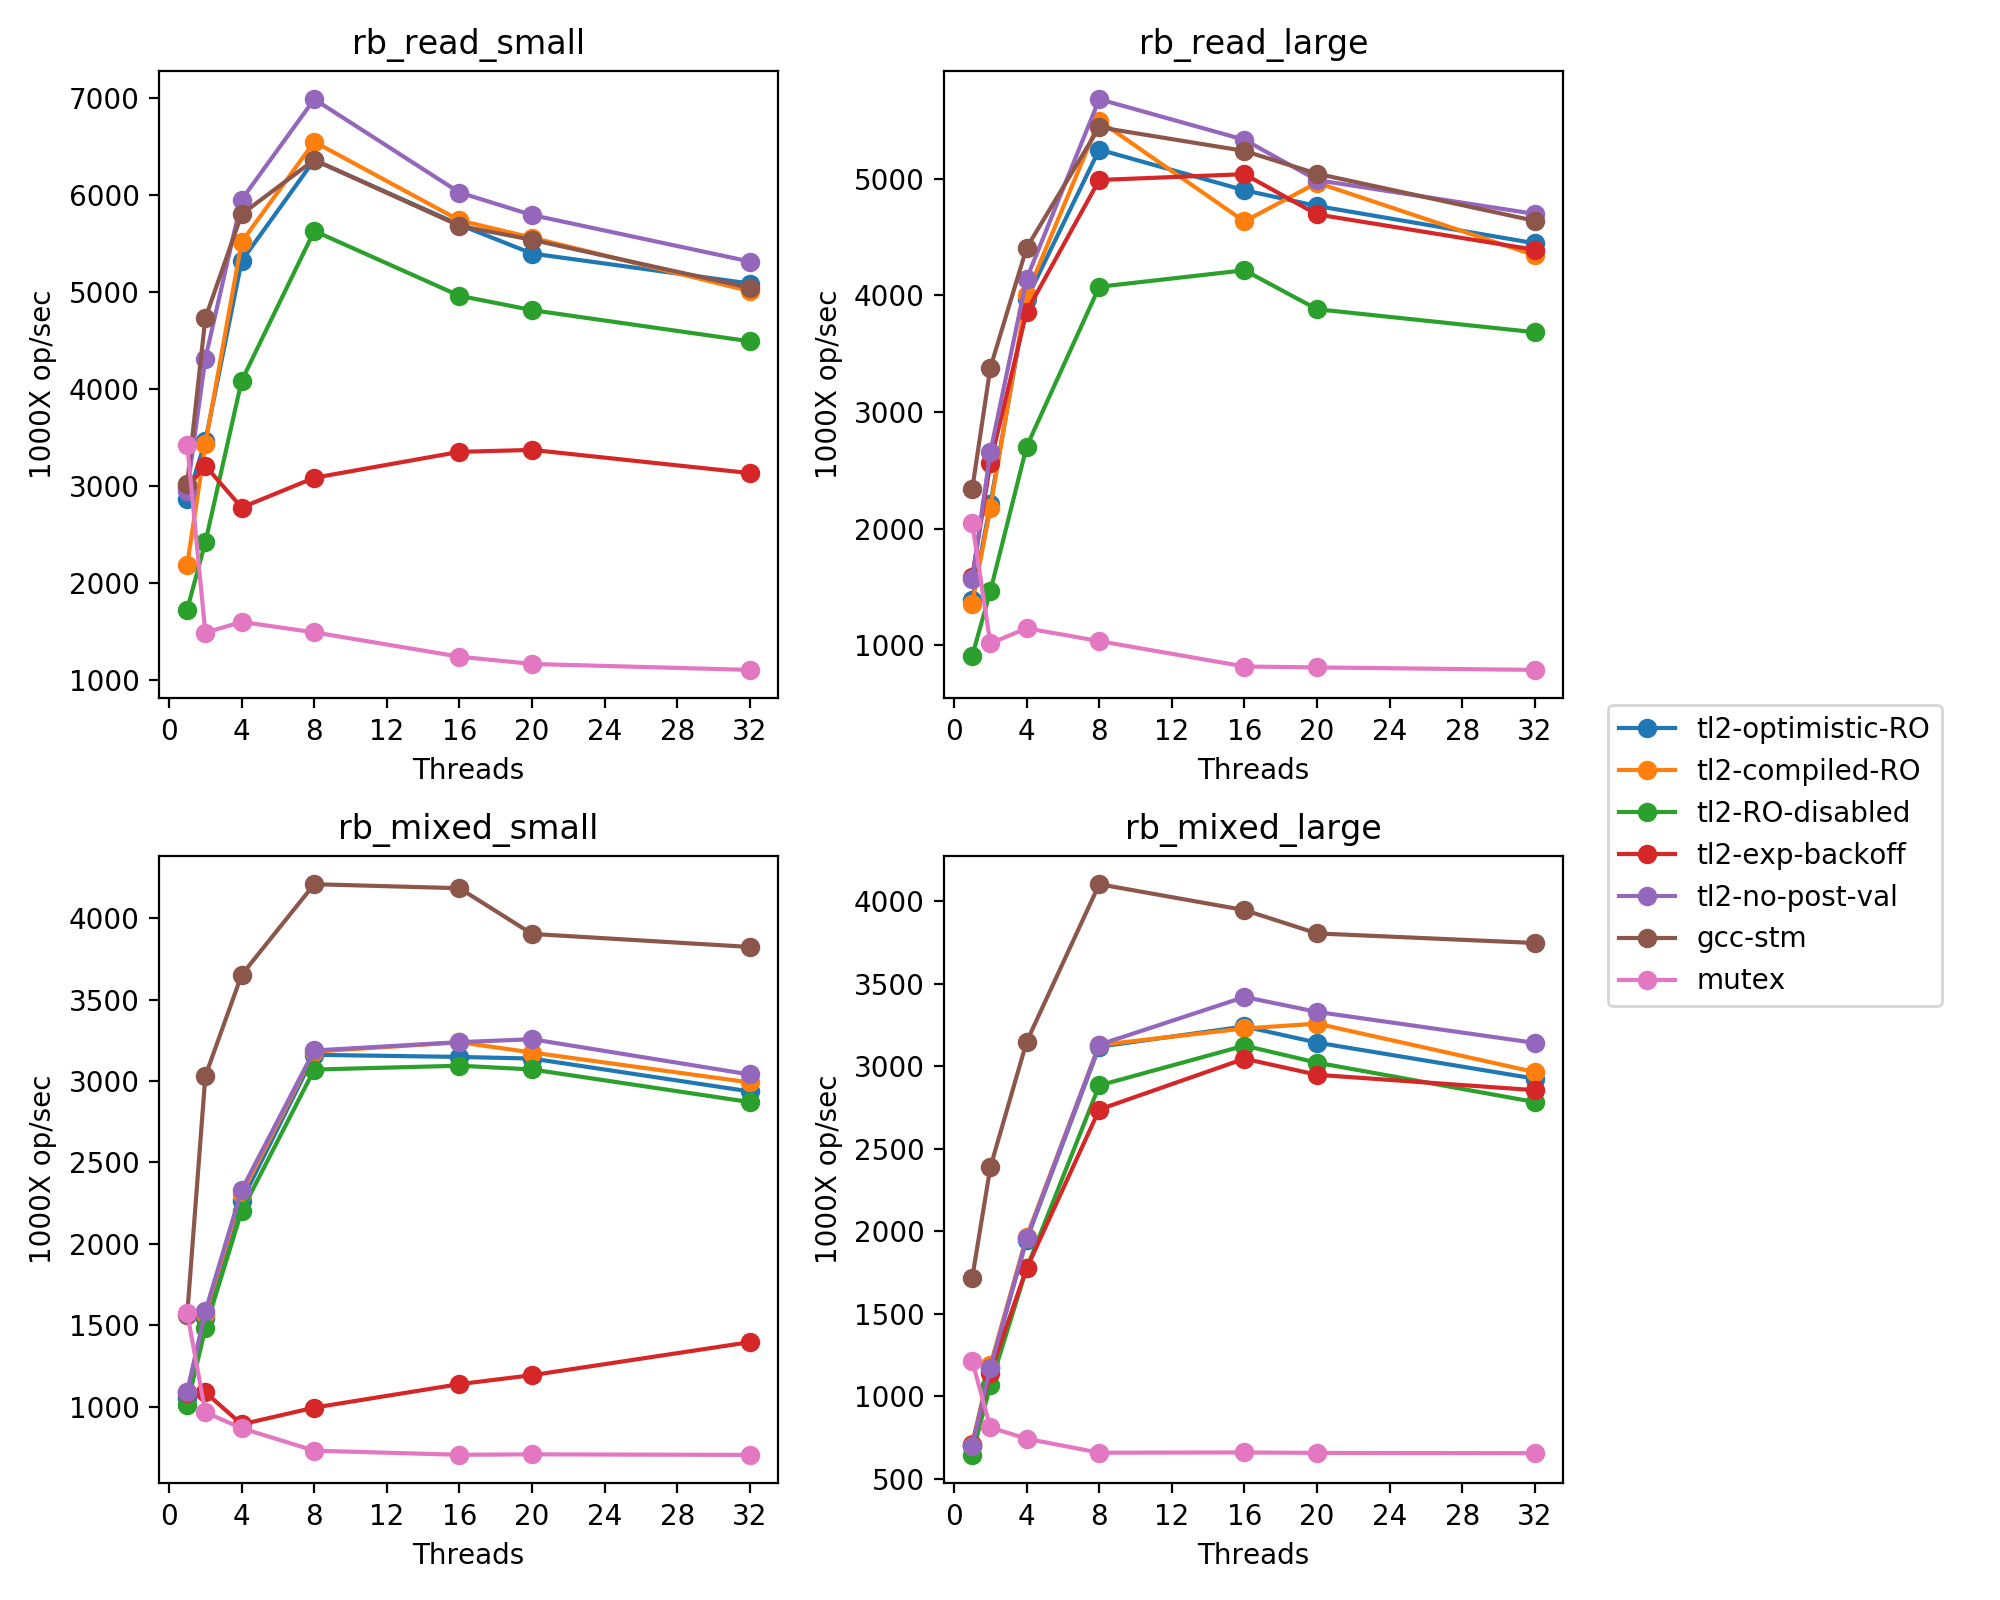
\includegraphics[width=\textwidth]{Sources/rb_graph (1).png}

\caption{TL2 speedup on selected STAMP benchmarks}
\label{GNN Execution Diagram}
\end{figure} 


%%%%%%%%%%%%%%%%%%%%%%%%%%%%%%%%%%%%%%%%%%%%%%%%%%%%%%%%%%%%%%%%%%%%%%%%
\section{Why?}
%%%%%%%%%%%%%%%%%%%%%%%%%%%%%%%%%%%%%%%%%%%%%%%%%%%%%%%%%%%%%%%%%%%%%%%%

I was not satisfied with the available templates for \LaTeX{} and wanted
to heed the style advice given by people such as Robert
Bringhurst~\cite{Bringhurst12} or Edward R.\
Tufte~\cite{Tufte90,Tufte01}. While there \emph{are} some packages out
there that attempt to emulate these styles, I found them to be either
too bloated, too playful, or too constraining. This template attempts to
produce a beautiful look without having to resort to any sort of hacks.
I hope you like it.

%%%%%%%%%%%%%%%%%%%%%%%%%%%%%%%%%%%%%%%%%%%%%%%%%%%%%%%%%%%%%%%%%%%%%%%%
\section{How?}
%%%%%%%%%%%%%%%%%%%%%%%%%%%%%%%%%%%%%%%%%%%%%%%%%%%%%%%%%%%%%%%%%%%%%%%%

The package tries to be easy to use. If you are satisfied with the
default settings, just add
%
\begin{verbatim}
\documentclass{mimosis}
\end{verbatim}
%
at the beginning of your document. This is sufficient to use the class.
It is possible to build your document using either \LaTeX|, \XeLaTeX, or
\LuaLaTeX. I personally prefer one of the latter two because they make
it easier to select proper fonts.

%%%%%%%%%%%%%%%%%%%%%%%%%%%%%%%%%%%%%%%%%%%%%%%%%%%%%%%%%%%%%%%%%%%%%%%%
\section{Making this template \emph{yours}}
%%%%%%%%%%%%%%%%%%%%%%%%%%%%%%%%%%%%%%%%%%%%%%%%%%%%%%%%%%%%%%%%%%%%%%%%

Prior to using this template, the first thing you want to do is probably
a little bit of customisation. You can achieve quick changes in look and
feel by picking your own fonts. With the \verb|fontspec| package loaded
and  \XeLaTeX or \LuaLaTeX as your compiler, this is pretty simple:
%
\begin{verbatim}
\setmainfont{Your main font}
\setsansfont{Your sans-serif font}
\setmonofont{Your monospaced font}
\end{verbatim}
%
Make sure to select nice combinations of that are pleasing to
\emph{your} eyes---this is your document and it should reflect your own
style. Make sure to specify font names as they are provided by your
system. For instance, you might want to use the following combination:
%
\begin{verbatim}
\setmainfont{Libre Baskerville}
\setsansfont[Scale=MatchLowercase]{IBM Plex Sans}
\setmonofont[Scale=MatchLowercase]{IBM Plex Mono}
\end{verbatim}
%
\ifxetexorluatex
If these fonts exist on your system, your normal text will look
{\fontspec{Libre Baskerville}{a little bit different from the other font used
in this example PDF}}, while your sans-serif font {\fontspec[Scale=MatchLowercase]{IBM Plex Sans}will 
pair nicely with your} {\fontspec[Scale=MatchLowercase]{IBM Plex Mono}{monospaced font}}.
%
You can also remove the \verb|Scale| directive, but I find that most
fonts pair better if they are adjusted in size a little bit. Experiment
with it until you finds a combination that you enjoy.
\fi

%%%%%%%%%%%%%%%%%%%%%%%%%%%%%%%%%%%%%%%%%%%%%%%%%%%%%%%%%%%%%%%%%%%%%%%%
\section{Features}
%%%%%%%%%%%%%%%%%%%%%%%%%%%%%%%%%%%%%%%%%%%%%%%%%%%%%%%%%%%%%%%%%%%%%%%%

%%%%%%%%%%%%%%%%%%%%%%%%%%%%%%%%%%%%%%%%%%%%%%%%%%%%%%%%%%%%%%%%%%%%%%%%
\begin{table}
  \centering
  \begin{tabular}{ll}
    \toprule
    \textbf{Package}      & \textbf{Purpose}\\
    \midrule
      \texttt{amsmath}          & Basic mathematical typography\\
      \texttt{amsthm}           & Basic mathematical environments for proofs etc.\\
      \texttt{babel}            & Language settings\\
      \texttt{booktabs}         & Typographically light rules for tables\\
      \texttt{bookmarks}        & Bookmarks in the resulting PDF\\
      \texttt{csquotes}         & Language-specific quotation marks\\
      \texttt{dsfont}           & Double-stroke font for mathematical concepts\\
      \texttt{graphicx}         & Graphics\\
      \texttt{hyperref}         & Hyperlinks\\
      \texttt{multirow}         & Permits table content to span multiple rows or columns\\ 
      \texttt{paralist}         & Paragraph~(`in-line') lists and compact enumerations\\
      \texttt{scrlayer-scrpage} & Page headings\\
      \texttt{setspace}         & Line spacing\\
      \texttt{siunitx}          & Proper typesetting of units\\
      \texttt{subcaption} & Proper sub-captions for figures\\
    \bottomrule
  \end{tabular}
  \caption{%
    A list of the most relevant packages required~(and automatically imported) by this template.
  }
  \label{tab:Packages}
\end{table}
%%%%%%%%%%%%%%%%%%%%%%%%%%%%%%%%%%%%%%%%%%%%%%%%%%%%%%%%%%%%%%%%%%%%%%%%

The template automatically imports numerous convenience packages that
aid in your typesetting process. \autoref{tab:Packages} lists the
most important ones. Let's briefly discuss some examples below. Please
refer to the source code for more demonstrations.

%%%%%%%%%%%%%%%%%%%%%%%%%%%%%%%%%%%%%%%%%%%%%%%%%%%%%%%%%%%%%%%%%%%%%%%%
\subsection{Typesetting mathematics}
%%%%%%%%%%%%%%%%%%%%%%%%%%%%%%%%%%%%%%%%%%%%%%%%%%%%%%%%%%%%%%%%%%%%%%%%

This template uses \verb|amsmath| and \verb|amssymb|, which are the
de-facto standard for typesetting mathematics. Use numbered equations
using the \verb|equation| environment.
%
If you want to show multiple equations and align them, use the
\verb|align| environment:
%
\begin{align}
    V &:= \{ 1, 2, \dots \}\\
    E &:= \big\{ \left(u,v\right) \mid \dist\left(p_u, p_v\right) \leq \epsilon \big\}
\end{align}
%
Define new mathematical operators using \verb|\DeclareMathOperator|.
Some operators are already pre-defined by the template, such as the
distance between two objects. Please see the template for some examples. 
%
Moreover, this template contains a correct differential operator. Use \verb|\diff| to typeset the differential of integrals:
%
\begin{equation}
  f(u) := \int_{v \in \domain}\dist(u,v)\diff{v}
\end{equation}
%
You can see that, as a courtesy towards most mathematicians, this
template gives you the possibility to refer to the real numbers~$\real$
and the domain~$\domain$ of some function. Take a look at the source for
more examples. By the way, the template comes with spacing fixes for the
automated placement of brackets.

%%%%%%%%%%%%%%%%%%%%%%%%%%%%%%%%%%%%%%%%%%%%%%%%%%%%%%%%%%%%%%%%%%%%%%%%
\subsection{Typesetting text}
%%%%%%%%%%%%%%%%%%%%%%%%%%%%%%%%%%%%%%%%%%%%%%%%%%%%%%%%%%%%%%%%%%%%%%%%

Along with the standard environments, this template offers
\verb|paralist| for lists within paragraphs.
%
Here's a quick example: The American constitution speaks, among others, of
%
\begin{inparaenum}[(i)]
  \item life
  \item liberty
  \item the pursuit of happiness.
\end{inparaenum}
%
These should be added in equal measure to your own conduct. To typeset
units correctly, use the \verb|siunitx| package. For example, you might
want to restrict your daily intake of liberty to \SI{750}{\milli\gram}.

Likewise, as a small pet peeve of mine, I offer specific operators for
\emph{ordinals}. Use \verb|\th| to typeset things like July~4\th
correctly. Or, if you are referring to the 2\nd edition of a book,
please use \verb|\nd|. Likewise, if you came in 3\rd in a marathon, use
\verb|\rd|. This is my 1\st rule.

If you want to write a text in German and use German hyphenation rules, set the language of your text to german using \verb|\selectlanguage{ngerman}|, or add
\begin{verbatim}
\PassOptionsToPackage{spanish}{babel}
\end{verbatim}
before the \verb|\documentclass| command to load a specific language. The languages \verb|ngerman|, \verb|french|, and \verb|english| are loaded by default, with \verb|english| being selected.

Quotation marks can be typeset using the \verb|\enquote{...}| command from the \verb|csquotes| package, which is preloaded by \verb|latex-mimosis|.
Depending on the currently selected language, quotes will look like \enquote{this},
\selectlanguage{ngerman}\enquote{this}\selectlanguage{english},
or
\selectlanguage{french}\enquote{this}\selectlanguage{english}.
One must never use "ASCII" quotation marks or even 'apostrophe' symbols.

%%%%%%%%%%%%%%%%%%%%%%%%%%%%%%%%%%%%%%%%%%%%%%%%%%%%%%%%%%%%%%%%%%%%%%%%
\section{Changing things}
%%%%%%%%%%%%%%%%%%%%%%%%%%%%%%%%%%%%%%%%%%%%%%%%%%%%%%%%%%%%%%%%%%%%%%%%

Since this class heavily relies on the \verb|scrbook| class, you can use
\emph{their} styling commands in order to change the look of things. For
example, if you want to change the text in sections to \textbf{bold} you
can just use
%
\begin{verbatim}
  \setkomafont{sectioning}{\normalfont\bfseries}
\end{verbatim}
%
at the end of the document preamble---you don't have to modify the class
file for this. Please consult the source code for more information.
